\documentclass[hidelinks,12pt]{article}

\usepackage{lmodern}
\usepackage[utf8]{inputenc}
\usepackage[T1]{fontenc}
\usepackage[french]{babel}
\usepackage{url}
\usepackage{graphicx}
\usepackage{pifont}
\usepackage{subfig}
\usepackage{listings}
\usepackage{changepage}
\usepackage{hyperref}

\graphicspath{ {./img/} }

\newcommand{\cmark}{\ding{51}}
\newcommand{\xmark}{\ding{55}}

\title{\textbf{Analyse de données d’eye-tracking en Réalité Virtuelle}}
\author{\Large{Adonis Stavridis}}
\date{Mai 2021}

\begin{document}

% ------------------------------------------------------------------------------
% TITLEPAGE
% ------------------------------------------------------------------------------

\maketitle
\tableofcontents
\pagebreak

% ------------------------------------------------------------------------------
% INTRODUCTION
% ------------------------------------------------------------------------------

\section{Introduction}

L'eye-tracking \cite{wiki_eye_tracking}, ou oculométrie, est une technologie
qui permet de reconnaître la position du regard d'un individu dans un
environnement virtuel ou réel. Elle fournit un moyen de suivre les processus
attentionnels d'un utilisateur et permet d'établir une interface entre
Homme et machine. Cette technique peut être très utilisée pour les études liées
au système visuel humain, à la psychologie, au marketing et au design. Elle est
en fait dèjà utilisée dans les jeux vidéos. Bien que cette technologie soit
bien connue et employée dans multiples domaines de recherche, elle est encore
peu exploitée dans le domaine de la réalité virtuelle.

\bigskip
Déterminer la position du regard d'un individu dans un environnement permet
d'effectuer des études quantitatives et qualitatives sur de multiples supports,
et ainsi, de comprendre les cognitions et comportements humains dans différentes
situations. L'eye-tracking s'avère donc être très pratique pour étudier la
saillance des éléments présents dans les environnements virtuels. Cependant,
certaines études ont besoin d'un environnement plus réaliste. La réalité
virtuelle ajoute une nouvelle couche d'immersion, permettant à un individu de
se sentir et agir de façon plus réaliste. La réalité virtuelle permettrait
alors de livrer des résultats beaucoup plus fiables pour certains domaines, et
ainsi pousser à l'avancement des recherches sur le comportement humain.

\bigskip
L'objectif de ce travail consiste à développer un outil d'analyse des données
d'oculométrie afin de comparer le regard face à un écran et dans un
environnement de réalité virtuelle. La visualisation et l'analyse des données
oculaires, peut être effectuée en temps réel ou par l'intermédiaire d'une
application. En vue de ce travail de recherche, un premier environnement (cf.
Figure \ref{fig:environnement}) a déjà été mis au point pour recueillir des
données d'eye-tracking sur un écran d'ordinateur, mais aussi dans un
environnement de réalité virtuelle. Un individu se place devant un écran et
observe différents supports, quant à la réalité virtuelle, l'individu porte un
casque et se retrouve dans ce même environnement face à un écran, cette fois-ci,
dans un monde virtuel. A partir des données recueillies au cours de sessions
expérimentales, il faudrait générer des supports graphiques qui rassemblent
toutes les informations nécessaires pour une analyse compléte de l'étude. Il
existe certaines bibliothèques et logiciels qui permettent de traiter ces
données, mais toutes ne présentent pas les mêmes fonctionnalités.

\begin{figure}[htpb]
  \centering
  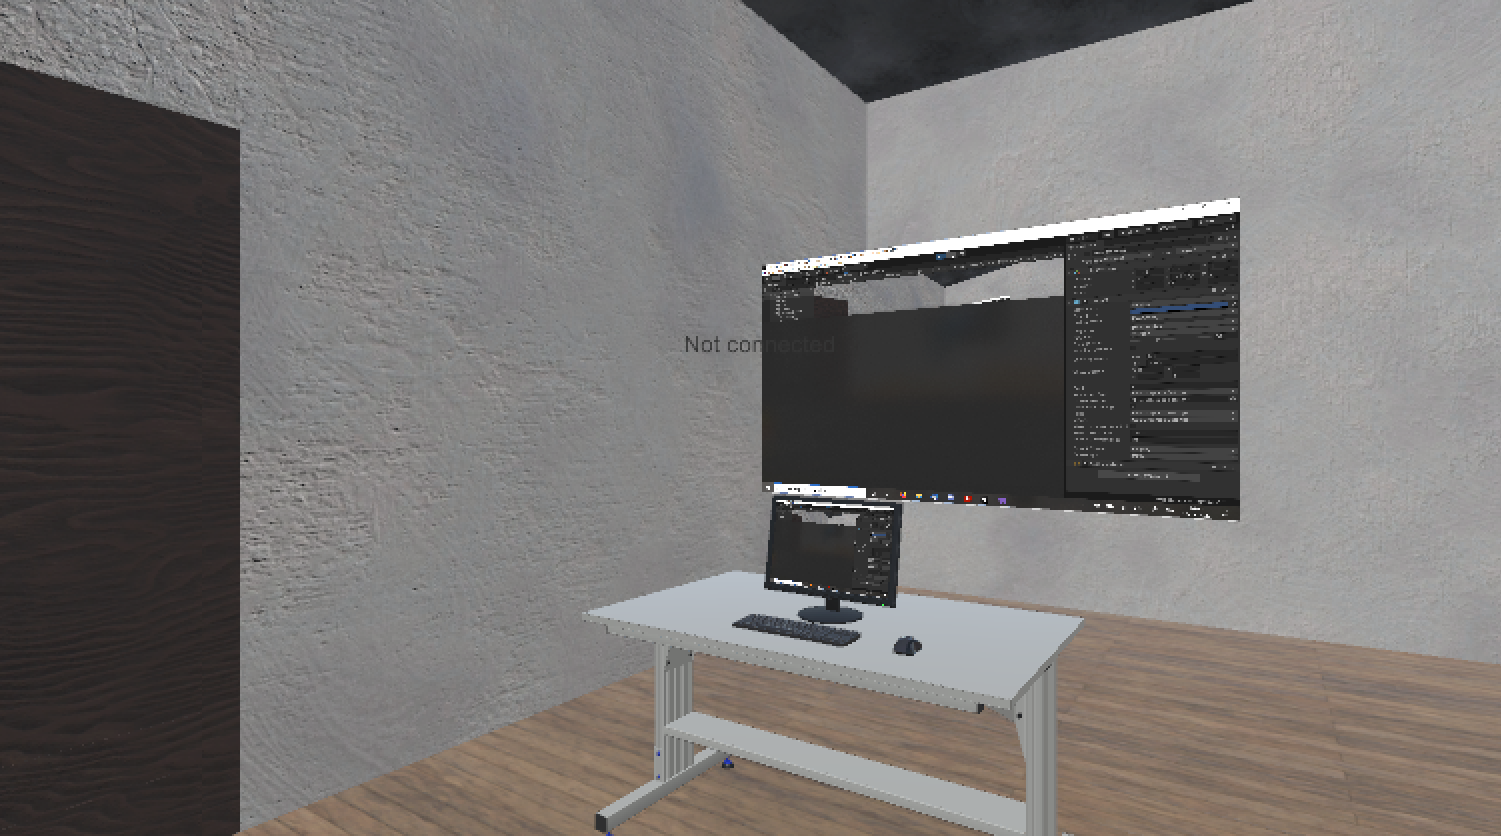
\includegraphics[width=0.75\textwidth,keepaspectratio=true]{environnement.png}
  \caption{Rendu de l'environnement mis en place en réalité virtuelle pour
    effectuer des mesures d'oculométrie \cite{img_environnement}.}
  \label{fig:environnement}
\end{figure}

\bigskip
Il convient dans un premier temps de sélectionner l'outil qui possède les
meilleurs atouts pour réaliser ces supports. Pour cela, il faut d'abord
comprendre comment sont récupérées les données, comment elle sont structurées
et puis identifier les types de support pertinents pour une analyse compléte,
afin de déterminer la bibliothèque la plus intéressante à utiliser pour
accomplir ce travail. Enfin, il faut programmer cet outil et vérifier que les
résultats obtenus sont cohérents avec les données d'entrée.

% ------------------------------------------------------------------------------
% CAPTEURS
% ------------------------------------------------------------------------------

\section{Capteurs}

L'eye-tracking est permis grâce à des émetteurs spéciaux qui envoient des rayons
infrarouges, non perceptibles par l'œil humain, vers les yeux d'un individu.
Ces rayons sont alors réfléchis par les yeux et les capteurs, à leur réception,
calculent la direction du regard. Grâce à un logiciel intégré aux capteurs, le
dispositif va déterminer la position du regard dans un environnement d'étude,
que ce soit un écran ou un monde virtuel.

\bigskip
Les deux types de capteurs utilisés au sein de ce travail sont les suivants :
\begin{itemize}
  \item Des capteurs pour écrans : ce sont les capteurs les plus basiques. Ils
        sont placés au-dessus ou en-dessous d'un écran et orientés vers les yeux
        d'un individu. Ils permettent de suivre le regard sur un écran, donc
        dans un environnement à deux dimensions.
  \item Des capteurs intégrés à des casques de réalité virtuelle : ce sont des
        capteurs similaires aux précédents, mais qui ont été modifiés pour
        s'intégrer dans des casques de réalité virtuelle et observer les yeux à
        une distance beaucoup plus courte. Ces capteurs permettent de suivre le
        regard dans un environnement virtuel à trois dimensions. Ce type de
        capteur peut poser plusieurs avantages tel que le rendu fovéal
        \cite{wiki_foveated_rendering}.
\end{itemize}

\bigskip
La plupart des produits liés à l'eye-tracking sont distribués par des
entreprises telles que Tobii \cite{tobii} et HTC Vice \cite{htc_vive_pro_eye}.
Ces solutions peuvent être utilisées dans plusieurs domaines \cite{yt_tobii_vr}
: les capteurs pour écrans peuvent être utiles pour étudier le regard d'un
individu sur une page web, par exemple, et ainsi déterminer les régions les
plus attrayantes ou non. Les casques de réalité virtuelle avec capteurs
intégrés sont quant à eux utilisés dans des situations d'entraînement ou des
circonstances difficilement réalisables dans le monde réel.

\begin{figure}[htpb]
  \centering
  \subfloat{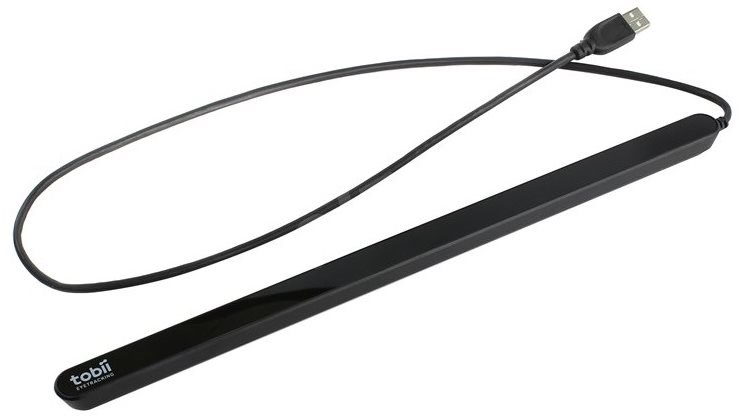
\includegraphics[width=6cm]{tobii.jpeg}}
  \qquad
  \subfloat{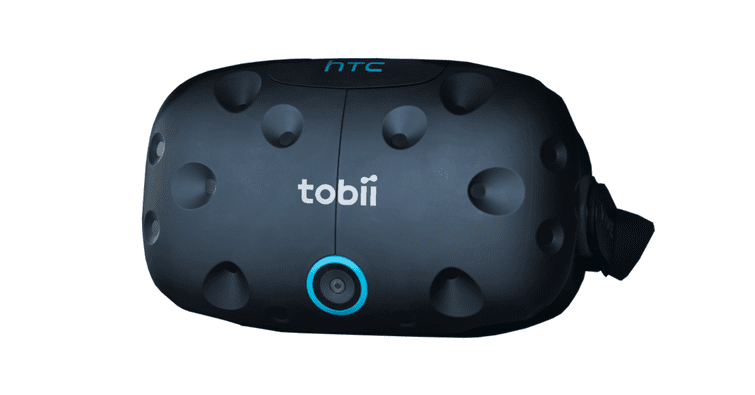
\includegraphics[width=6cm]{htcvive.png}}
  \caption{Capteur Tobii \cite{img_tobii} pour écrans (à gauche) et casque HTC
    Vive \cite{img_htcvive} pour la réalité virtuelle (à droite).}
  \label{fig:materiel}
\end{figure}

Il existe plusieurs types de capteurs, certains plus spécialisés dans certains
domaines que d'autres. Les capteurs sont fournis avec des logiciels capables de
produire toutes les données nécessaires pour les analyser. Dans le cadre de ce
travail, les capteurs utilisés sont une barre de tracking Tobii pour écrans et
un casque HTC Vive avec capteur intergré pour la réalité virtuelle (cf. Figure
\ref{fig:materiel}).

% ------------------------------------------------------------------------------
% ANALYSE DES DONNÉES
% ------------------------------------------------------------------------------

\section{Analyse des données}

Après avoir récupéré les données brutes d'une séance d'oculométrie, il faut
pouvoir les analyser afin d'en tirer des informations pertinentes. Les
données sont une série de valeurs numériques (cf. Figure \ref{fig:donnees}),
représentants essentiellement les positions du regard dans un environnement,
mais sont difficilement compréhensibles telles quelles. Pour cela, il serait
beaucoup plus intéressant de transformer les données en des réprésentations
graphiques dont on distingue les régions d'intérêt facilement. Il existe
différentes mesures et termes  utilisés pour analyser le regard
\cite{imotions_metrics}, chacune organisant les données de façon à avoir une
analyse compléte, étudiant tous les aspects du regard.

\begin{figure}[htpb]
  \begin{lstlisting}
    <temps> : <positionX>, <positionY>
    0.00 : 50, 50
    0.25 : 43, 64
    0.50 : 38, 75
    0.75 : 41, 66
    ...
  \end{lstlisting}
  \caption{Exemple de données fournies par les logiciels de capteurs, avec une
    indication du temps et de la position du regard (en pourcentages) sur l'axe
    horizontal et vertical.}
  \label{fig:donnees}
\end{figure}

\subsection{Points de fixation}

L'un des indicateurs les plus utilisés pour représenter le regard au fil du
temps sont les points de fixation. Ce sont des mesures qui consistent à indiquer
le point de focalisation d'un individu à un instant donné. Un capteur qui
collectionne des données avec un taux d'échantillonage de 120hz, par exemple, va
fournir en sortie 120 points de fixation par seconde. Il faut donc faire une
organisation de ces points en fonctions du temps et de l'espace. La quantité de
points de fixation montre à quel point l'attention visuelle a été portée en une
région.

\subsection{Séquence de fixations}

Étudier la séquence de ces points de fixations serait également intéressant. Un
individu va d'abord fixer son regard sur les régions les plus prioritaires et va
se construire l'environnement petit à petit, en se concentrant sur plusieurs
zones. L'ordre d'attention est important dans la recherche car elle reflète de
l'intérêt d'un individu sur une région et met en avant les objets les plus
captivants au premier regard. Le premier point de fixation peut être aléatoire,
mais les zones de fixations qui suivent peuvent parfois être prédites, pour
une interface utilisateur, par exemple.

\subsection{Carte de chaleur}

Une autre représentation très importante est la distribution des points de
fixation, sous la forme d'une carte de chaleur ou heatmap. Un gradient de
couleur est placé sur l'environnement original indiquant du rouge au bleu les
régions les plus attrayantes (cf. Figure \ref{fig:heatmap}). Ces heatmaps sont
un moyen très simple de différencier les régions qui attirent le plus
l'attention. C'est l'une des représentations les plus efficaces pour comprendre
la saillance des éléments dans un environnement.

\begin{figure}[htpb]
  \centering
  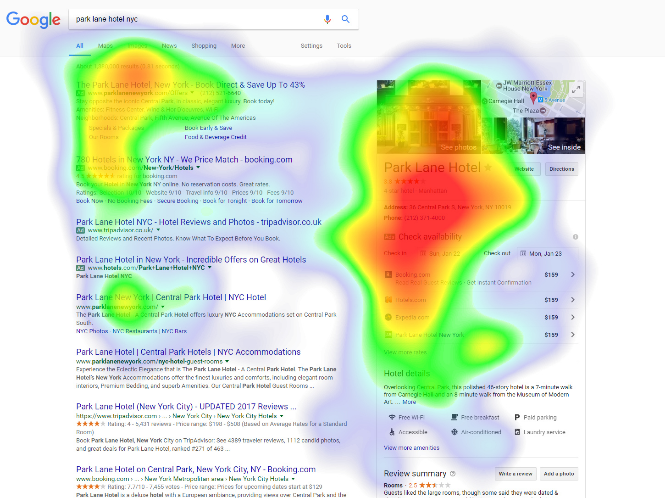
\includegraphics[width=0.75\textwidth,keepaspectratio=true]{heatmap.png}
  \caption{Exemple de heatmap sur une page de recherche sur Google
    \cite{img_heatmap}.}
  \label{fig:heatmap}
\end{figure}

\bigskip
Il existe donc plusieurs façons d'organiser les données et de les représenter
pour faciliter leur compréhension et permettre d'en tirer les bonnes
conclusions, en prenant en compte tous les aspects de l'étude du regard.

% ------------------------------------------------------------------------------
% LOGICIELS
% ------------------------------------------------------------------------------

\section{Logiciels}

Pour pouvoir analyser les données et créer ces réprésentations il faudrait soit
utiliser des bibliothèques ou des applications déjà disponibles
\cite{imotions_software}, soit créer les outils. Heureusement, il existe
certains logiciels open-source, ou gratuits uniquement, permettant d'effectuer
un minimum d'analyse de données. L'objectif est donc de déterminer quel
logiciel est le plus intéressant à utiliser dans le cadre de ce travail,
pour étudier le regard sur un écran, mais aussi dans un environnement de
réalité virtuelle.

\subsection{GazePointer}

Gazepointer \cite{gazepointer} est une application libre qui permet d'effectuer
de l'eye-tracking principalement. Il existe une fonctionnalité intégrée au
logiciel qui permet d'effectuer des séances de suivi du regard, et génerer une
heatmap des fixations. Cependant c'est la seule analyse possible. De plus,
c'est un logiciel qui fonctionne indépendamment, et non pas une bibliothèque :
ses outils ne sont pas accessibles en dehors de l'application. Aussi, le
logiciel fonctionne uniquement avec des webcams. Gazepointer permet d'analyser
des données d'oculométrie, mais son implémentation n'est pas optimale dans le
cadre de ce travail, avec les capteurs disponibles, et ne permet pas du tout
l'oculométrie en réalité virtuelle.

\subsection{Ogama}

Ogama \cite{ogama} est une application open-source qui permet d'enregistrer et
d'analyser des données d'oculométrie et de mouvements de souris. Le logiciel
permet essentiellement de créer des cartes de fixations et des zones d'intérêt,
et du calcul de saillance, pour déterminer quelles régions sont les plus
attrayantes. Il accepte tout type de données enregistrées en format ASCII, et,
en plus, le logiciel est certifié de fonctionner avec plusieurs logiciels
d'oculométrie et capteurs sur le marché tels que Tobii. Ogama est donc
certainement intéressant pour pouvoir importer et analyser des données
facilement. Cependant, ce n'est pas une bibliothèque et ne permet donc pas
beaucoup de flexibilité.

\subsection{PyGaze}

PyGaze \cite{pygaze} est quant à elle une boîte à outil Python, permettant
également d'effectuer du suivi de regard et de l'analyse des données. La
fonctionnalité la plus intéressante de cette bibliothèque est l'outil
de création de cartes. PyGaze permet d'afficher les données sous forme de
cartes de fixations et de chaleur. Le code de PyGaze est open-source et il est
donc possible de se baser sur cette bibliothèque pour développer d'autres
outils. De plus, elle est certifié de fonctionner avec les données issues de
capteurs Tobii. PyGaze est donc assez flexible et peut être utilisée ou
modifiée si nécessaire, pour obtenir des résultats d'analyse en fonction de nos
besoins.

\subsection{GazeParser}

GazeParser \cite{gazeparser} est une bibliothèque d'analyse des données du
regard qui permet essentielment de récupérer les données et les visualiser sous
forme de graphiques. Ceci peut être pratique pour avoir une approche plus brute
des données. GazeParser permet aussi d'appliquer des filtres sur les données
pour réduire le bruit et effectuer une analyse plus correcte. Même si ce format
d'analyse peut être intéressant, il ne rentre pas dans le cadre de ce travail.

\bigskip
\begin{table}[htpb]
  \begin{center}
    \begin{tabular}{|c||c|c|c|}
      \hline
      \multicolumn{4}{|c|}{Comparaison des logiciels}             \\
      \hline
      Logiciels   & Flexibilité   & Analyse       & Documentation \\
      \hline
      GazePointer & \xmark        & \cmark        & \cmark        \\
      Ogama       & \xmark        & \cmark \cmark & \cmark        \\
      PyGaze      & \cmark \cmark & \cmark \cmark & \cmark \cmark \\
      GazeParser  & \cmark        & \cmark \cmark & \cmark        \\
      \hline
    \end{tabular}
    \caption{Comparaison des logiciels en fonction de leur flexibilité, leur
      capacité de géneration de d'analyse des données et leur documentation.}
    \label{tab:comparaison}
  \end{center}
\end{table}

Plusieurs applications et bibliothèques gratuites permettent d'effectuer une
analyse sur les jeux de données créés par les capteurs. Il existe également des
logiciels payants, mais ceux-ci sont hors de portée au sein de ce
travail. Après comparaison entre les logiciels (cf. Table \ref{tab:comparaison},
la bibliothèque PyGaze est idéale pour ce travail, puisque elle permettrait
d'être utilisée pour analyser les données librement et facilement, afin de
créer des réprésentations visuelles du regard au fil du temps.

% ----------------------------------------------------------------------------
% Outil d'analyse
% ----------------------------------------------------------------------------

\section{Outil d'analyse}

Afin de développer l'outil d'analyse \cite{github_ter}, il faut d'abord
comprendre comment la librairie PyGaze traite les données. Le format des
données en entrée peut varier en fonction des études. Durant ce travail, des
formats de données m'étaient fournis, l'un pour une étude avec un capteur sur
écran 2D et le second pour une étude en réalité virtuelle. La première étude a
été effectuée par une société tierce, tandis que la seconde a été conduite au
sein du laboratoire iCube, par mes encadrants, grâce à l'environnement
d'eye-tracking en réalité virtuelle qu'ils avaient mis en place. Pour ces
études-ci, dans les deux cas, on étudie le regard sur un écran, l'un dans la vie
réelle tandis que l'autre dans un monde virtuel. Les données à traiter sont
donc deux dimensionnelle et l'environnement importe peu ici.

\subsection{Implémentation}

La première fonctionnalité de l'outil est de convertir les données en entrée,
en des données compréhensibles et traitables par la suite. Puisque plusieurs
formats de données peuvent être passés en entrée, il faut configurer pour
chaque format comment traduire les données spécifiques à chaque étude, en un
format de données compréhensible par l'outil. Les données passées en entrée
sont essentielment un fichier csv et un ensemble d'images regroupés dans un
dossier spécifique. Le fichier csv contient les positions de points de fixation
au fur et à mesure d'une étude, la distance de l'individu par rapport à l'écran
et le diamètre de chaque pupille, par exemple. Mais certaines de ces
informations ne sont pas utilisée par l'outil. Ainsi, les données originales
sont transformées en des fichiers csv dont on connait la composition,
sous un format commun pour faciliter l'implémentation. Pour manipuler les
données d'entrée, il suffit de connaître le temps (en microsecondes), la
position des points de fixation en X et Y (en pourcentages), la distance de
l'individu face à l'écran (en mètres), et le diamètre de la pupille en chaque
œil (en millimètres). Une étude d'oculométrie est faite sur une séquence
d'image, donc il faut aussi faire correspondre les données aux images. Pour
cela, on peut indiquer à quel temps étudier une image spécifique. On peut donc
avoir un fichier csv contenant les données organisés sous le format de la Table
\ref{tab:format-csv} composée de deux sous-tables. Lorsque cette étape est
achevée, les données peuvent être analysées.

\bigskip
\begin{table}[htpb]
  \begin{adjustwidth}{0.05\textwidth}{0cm}
    \begin{tabular}{|c||c|}
      \hline
      Temps  & Image  \\
      \hline
      0.0    & image1 \\
      7.3    & image2 \\
      \vdots & \vdots \\
      \hline
    \end{tabular}
    \newline
    \begin{tabular}{|c||c|c|c|c|c|}
      \hline
      Temps  & Fixs/X & Fixs/Y & Distance & Pup/Gauche & Pup/Droite \\
      \hline
      0.0    & 43.2   & 57.8   & 0.5      & 2.8        & 2.8        \\
      4.7    & 34.4   & 49.6   & 0.4      & 2.8        & 2.8        \\
      8.1    & 30.7   & 52.1   & 0.4      & 2.8        & 2.8        \\
      \vdots & \vdots & \vdots & \vdots   & \vdots     & \vdots     \\
      \hline
    \end{tabular}
  \end{adjustwidth}
  \caption{Format des données d'un fichier csv après filtrage: le fichier est
    composé d'une première table indiquant le temps de début de chaque image et
    d'une seconde table contenant toutes les données de fixation.}
  \label{tab:format-csv}
\end{table}

Par la suite, il faut organiser ces données en des ensembles cohérents: une
étude est composée de plusieurs images, que l'on peut appeler scènes. Les
données de fixations n'affectent qu'une scène, donc un premier filtrage est
effectué pour associer à chaque scène les données qui lui sont pertinentes,
grâce à l'indicateur de temps. Après lecture du fichier csv rearrangé, on crée
les différentes scènes, chacune contenant l'image d'étude et l'ensemble des
points de fixation qui lui sont propres. Ces informations sont suffisantes pour
créer des représentations imagées du suivi du regard. Grâce à la bibliothèque
PyGaze l'outil lance alors le rendu en parallèle de cartes de chaleur et des
points de fixation pour chaque scène.

\bigskip
L'outil a tout de mêmes des limites: il n'effectue uniquement une
réorganisation des données et ensuite le rendu des scènes. Il y a malgrès tout
un filtrage  des valeurs erronées, des points de fixation qui se trouvent en
dehors d'une image, par exemple. Mais aucun traitement de données
supplémentaire n'est effectué pour l'instant, pour regrouper des points de
fixation proche en temps et espace. Aussi, puisqu'une étude peut
être effectuée sur une page web, on peut récupérer la donnée de scroll ou
défilement de la page. Cependant, pour la première étude je n'ai pas réussi à
proprement prendre en compte cette donnée, et donc les résultats d'analyse ne
sont pas totalement corrects, pour cette étude-ci. Les données peuvent être
récupérées de plusieurs façons différentes, donc l'implémentation de l'outil
doit tenir compte de cette flexibilité. Puisque cette étude en question a été
menée par une société tierce, l'échange d'information était lent aussi. C'est
un aspect de ce travail qui demandait plus de temps que prévu. Sinon, cette
version de l'outil reste tout de même complete et fonctionne bien avec des
pages statiques et des images.

\subsection{Résultats}

L'outil permet donc de générer des cartes de chaleur et de points de fixations.
Dans le cadre de ce travail, j'ai adapté l'outil pour fonctionner avec les
données fournies par la société tierce et celles de iCube également. L'outil est
utilisé à la fin d'une capture, donc l'environnement de travail est en fait non
pertinent, tant que les données sont complètes et traitables.

\bigskip
L'analyse de la première étude par l'outil retourne pour chaque scène une carte
de chaleur (cf. Figure \ref{fig:tea-resultats-heatmap}) et la carte des points
de fixations (cf. Figure \ref{fig:tea-resultats-raw}). On observe sur la carte
des points de fixations que les regions de l'image d'origine qui possèdent une
forte densité de points sont bien distinguées par la carte de chaleur.
Cependant, les données de défilement de page sont ignorées sur ces rendus de
cartes, et donc les cartes ne sont pas totalement fiables: les zones
d'intérêt sont bien placées sur l'axe horizontal mais pas forcément sur l'axe
vertical.

\bigskip
Quant à la seconde étude, menée dans une environnement de réalité virtuel,
l'outil effectue le rendu de chaque scène également. Ici, on observe une carte
des points de fixation (cf. Figure \ref{fig:vr-resultats-raw}) plus remplie:
les points sont en fait uniquement les positions brutes du regard au fil du
temps. Contrairement à l'étude précédente, aucun traitement des données n'a été
effectué avant l'analyse, pour regrouper les points de fixations par temps et
espace. On distingue donc toute les positions du regard. Cependant, on observe
plus clairement les zones attrayantes, surtout grâce à la carte de chaleur (cf.
Figure \ref{fig:vr-resultats-heatmap}). Pour cette étude, l'individu devait se
focaliser sur le titre de l'affiche, la date, l'endroit et l'organisateur de
l'événement. En étudiant ces cartes, on peut bien différencier les zones
reflettant ces informations.

\begin{figure}[htpb]
  \centering
  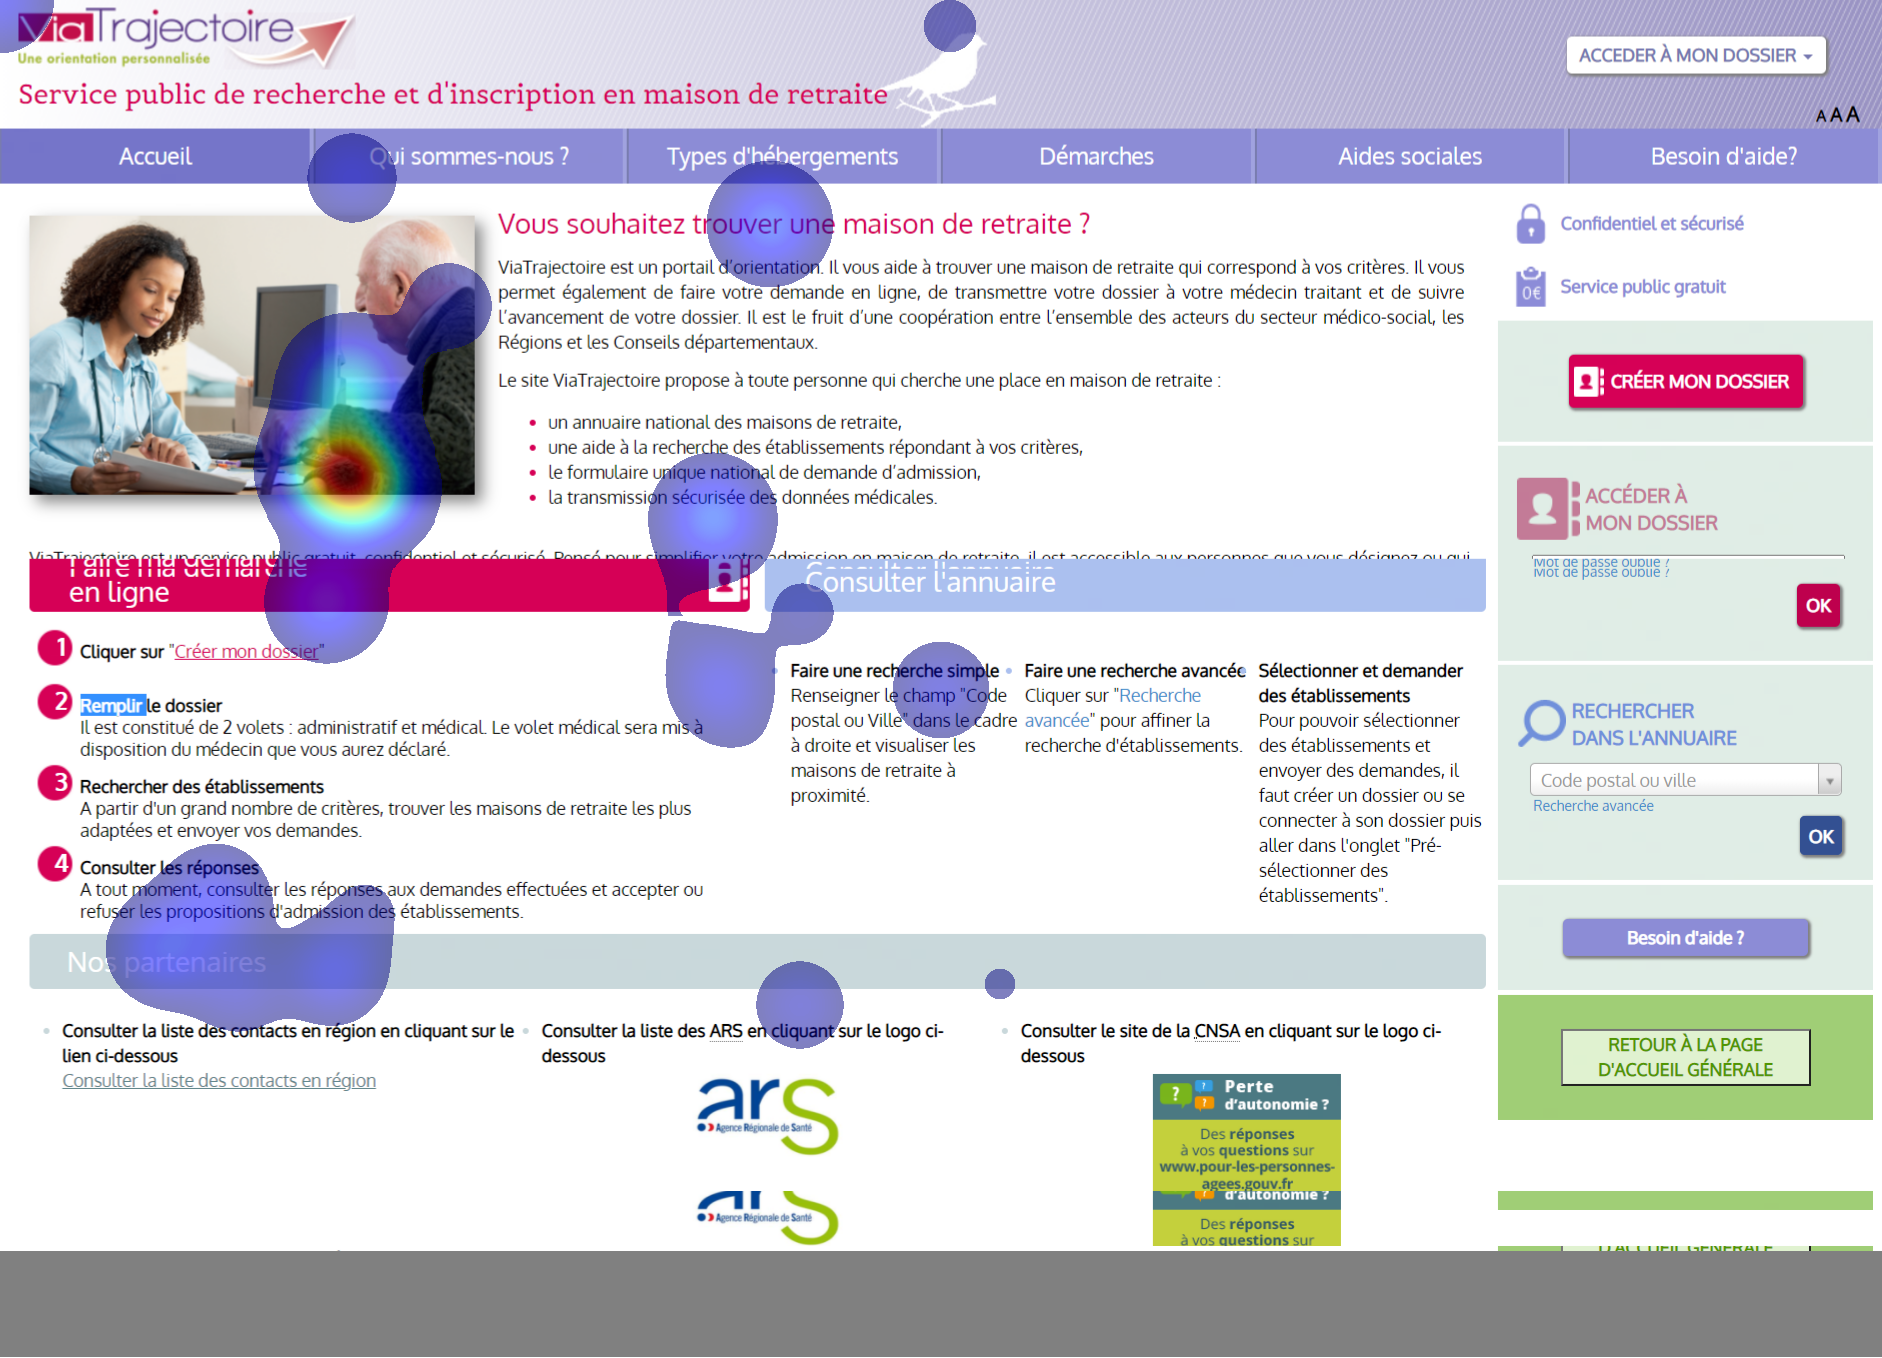
\includegraphics[width=0.8\textwidth,keepaspectratio=true]{tea-heatmap-9.png}
  \caption{Carte de chaleur générée à partir d'une étude effectuée avec un
    capteur d'écran 2D.}
  \label{fig:tea-resultats-heatmap}
\end{figure}

\begin{figure}[htpb]
  \centering
  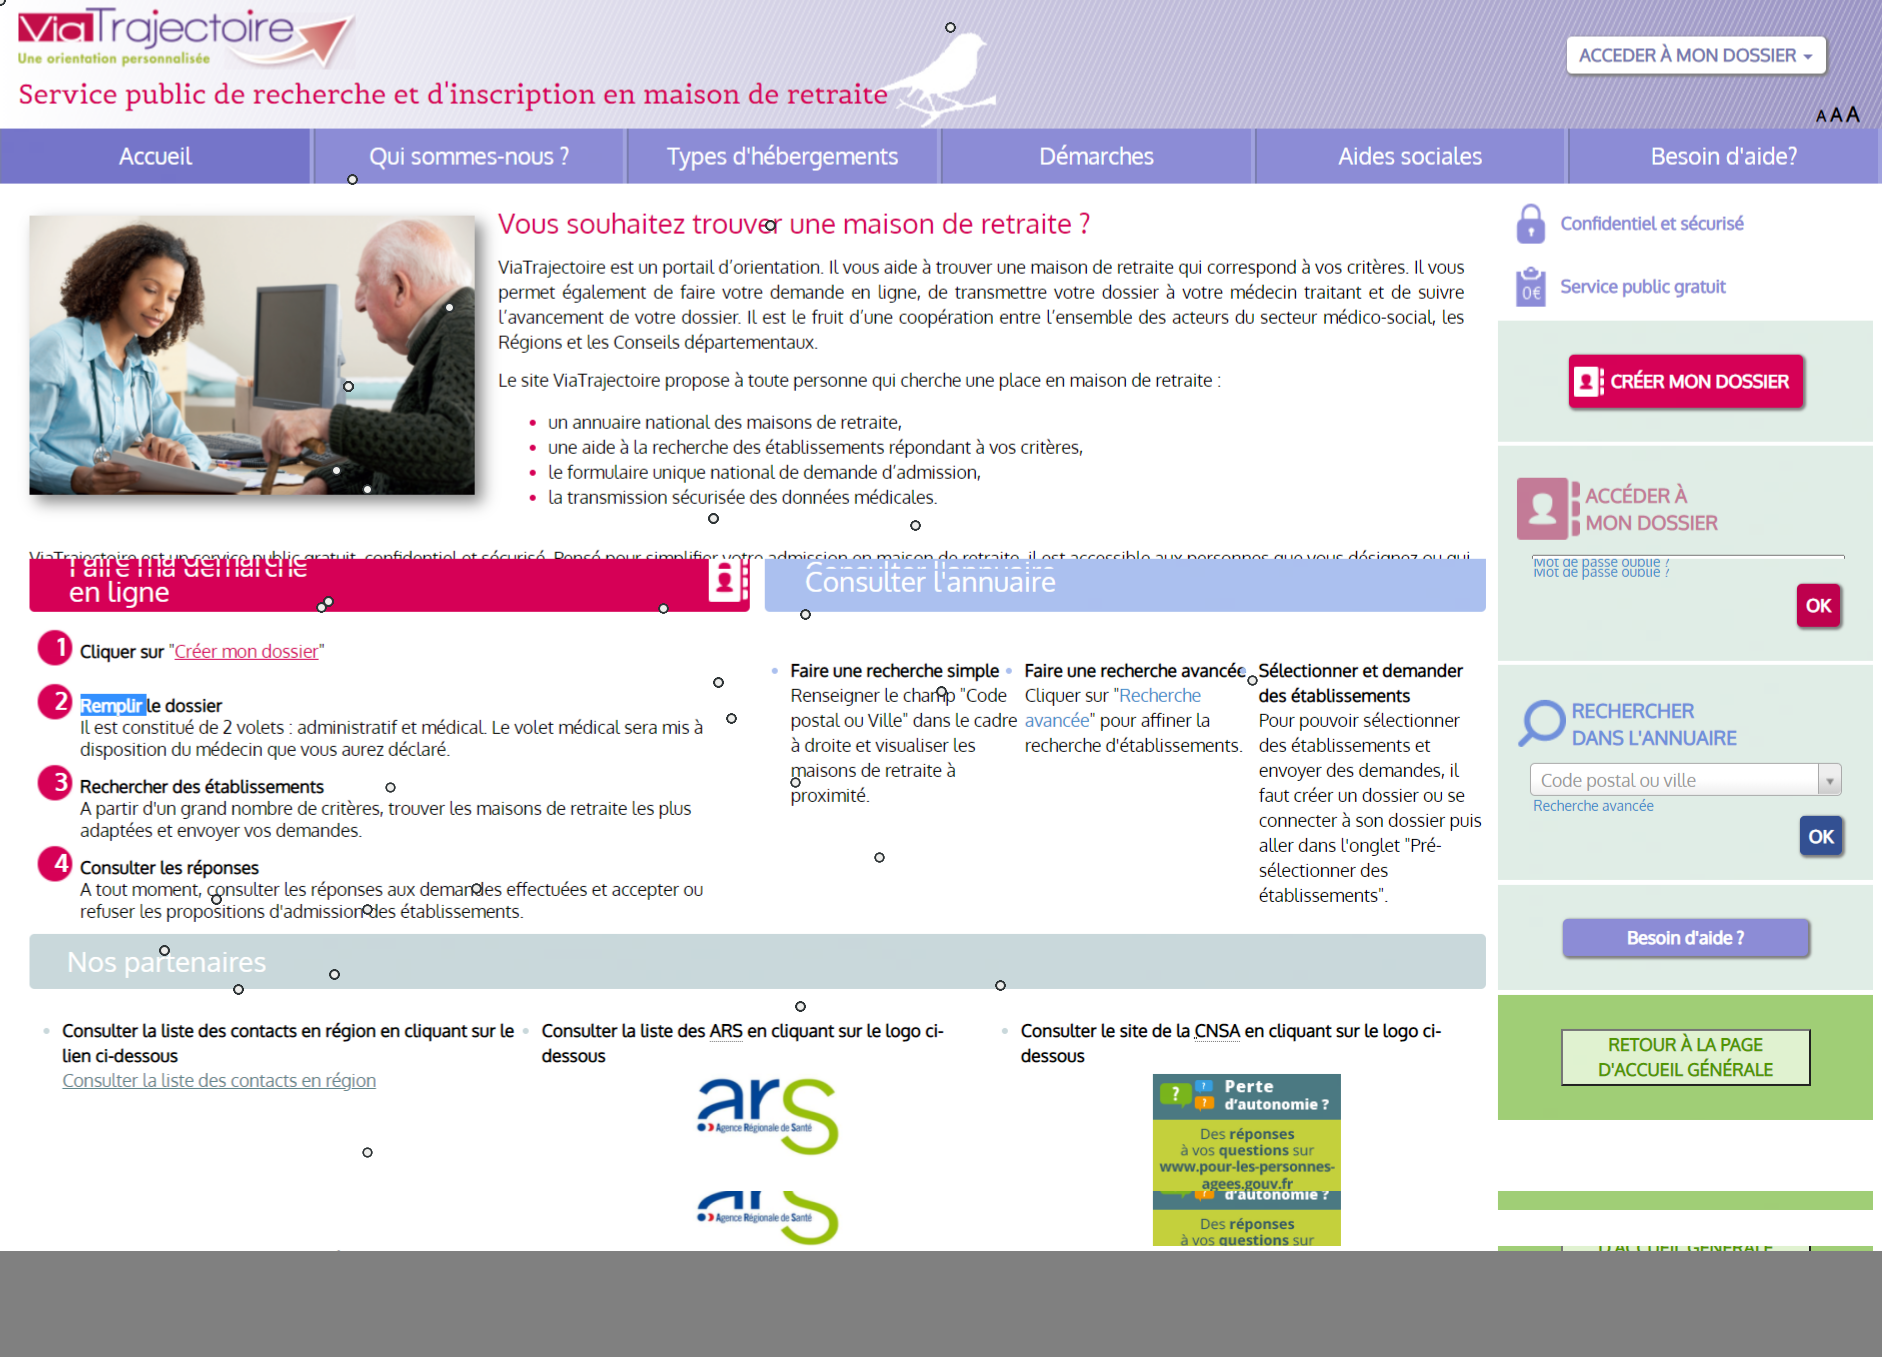
\includegraphics[width=0.8\textwidth,keepaspectratio=true]{tea-raw-9.png}
  \caption{Carte des points de fixation générée à partir d'une étude effectuée
    avec un capteur d'écran 2D.}
  \label{fig:tea-resultats-raw}
\end{figure}

\begin{figure}[htpb]
  \centering
  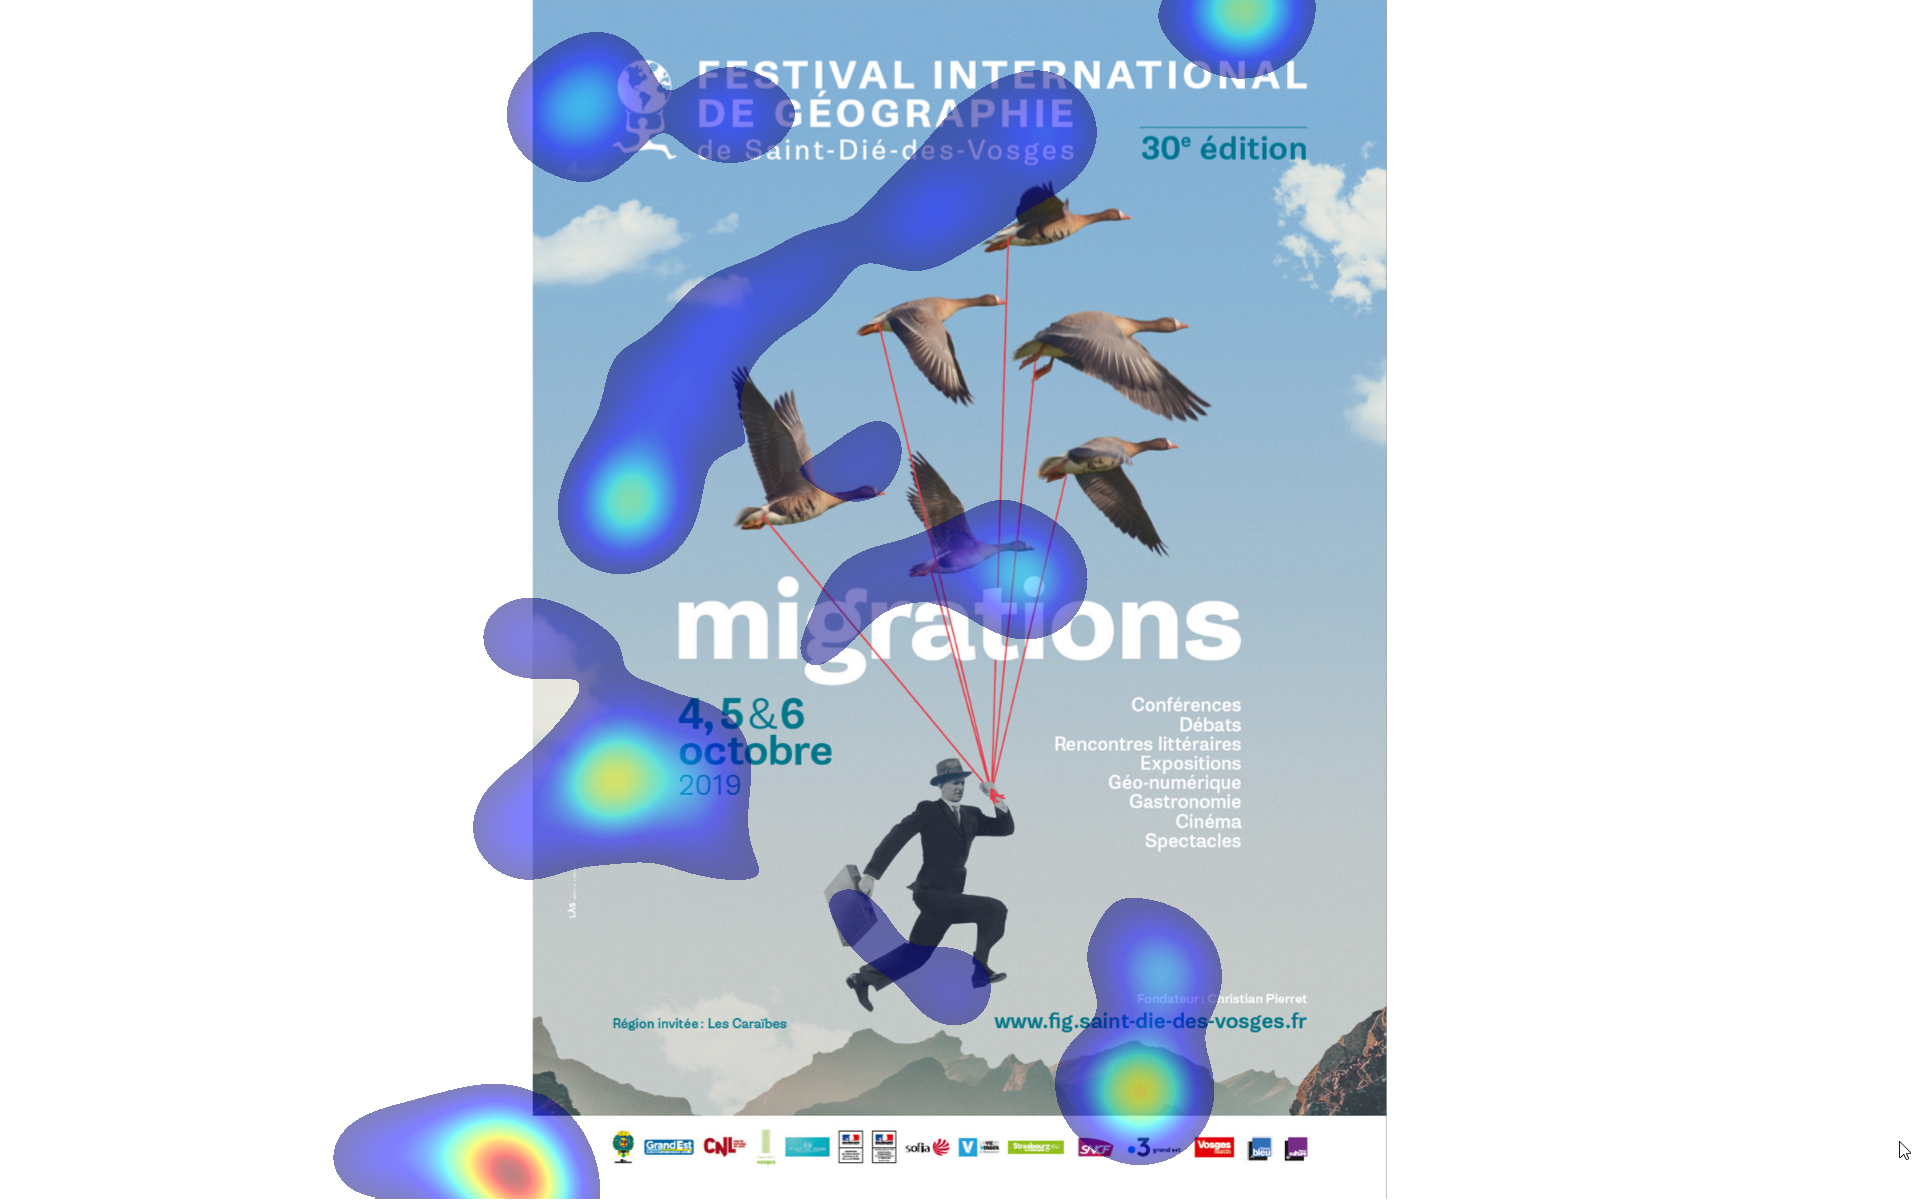
\includegraphics[width=0.8\textwidth,keepaspectratio=true]{vr-heatmap-0.png}
  \caption{Carte de chaleur générée à partir d'une étude effectuée avec un
    capteur de réalité virtuelle.}
  \label{fig:vr-resultats-heatmap}
\end{figure}

\begin{figure}[htpb]
  \centering
  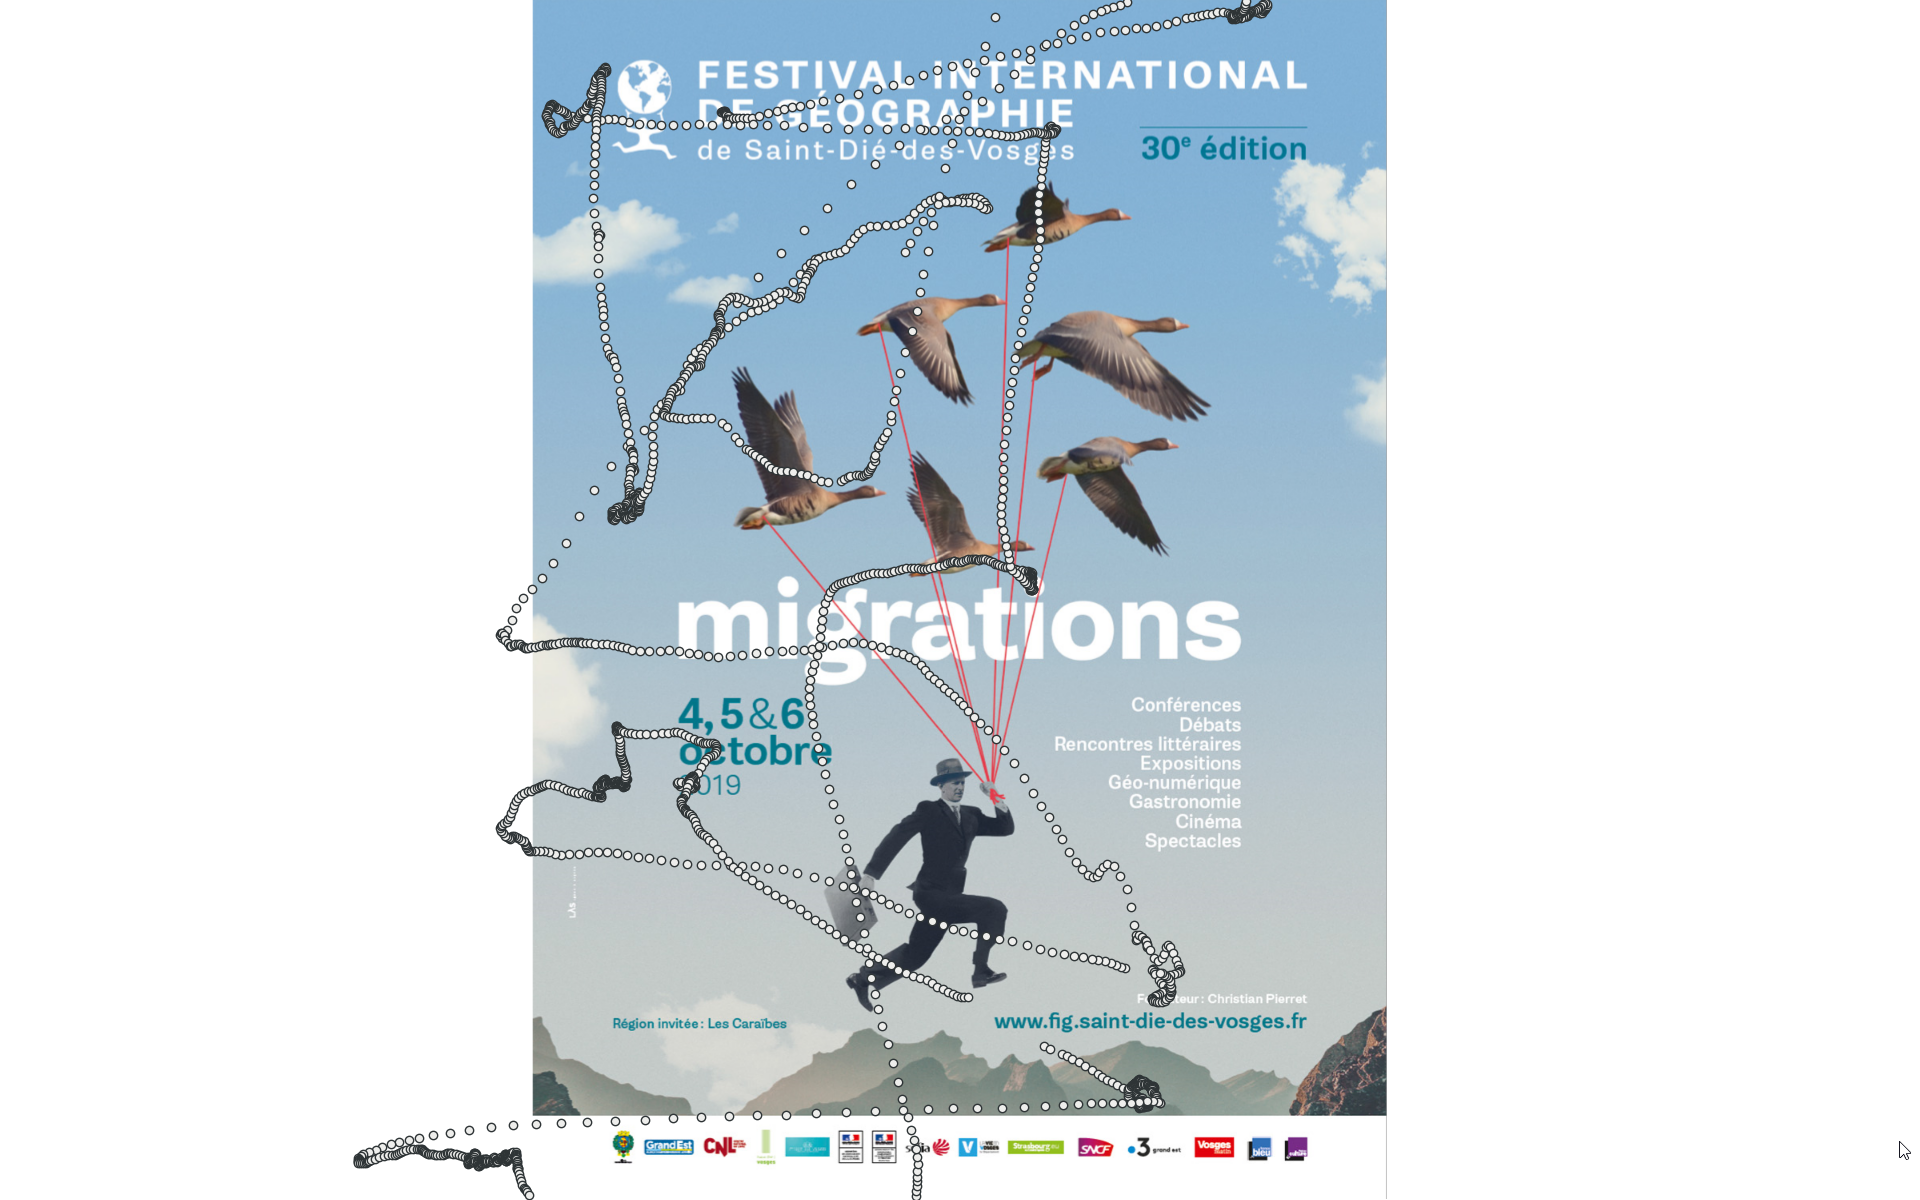
\includegraphics[width=0.8\textwidth,keepaspectratio=true]{vr-raw-0.png}
  \caption{Carte des points de fixation à partir d'une étude effectuée avec un
    capteur de réalité virtuelle.}
  \label{fig:vr-resultats-raw}
\end{figure}

\bigskip
Cet outil permet de créer des cartes qui facilitent l'analyse des données
d'oculométrie. Dans cette version fonctionnelle, il peut prendre en entrée deux
formats de données et les réorganiser pour effectuer le rendu des cartes
d'analyse. Ces cartes sont cohérentes avec les données d'entrée, même si
certaines fonctionnalités supplémentaires pourraient être ajoutées afin
d'analyser proprement des pages avec défilement et un prétraitement des données
pour n'afficher que les points de fixations. L'outil reste malgrès tout complet,
documenté, structuré en différentes classes et parallélisé aussi.


% ----------------------------------------------------------------------------
% CONCLUSION
% ----------------------------------------------------------------------------

\section{Conclusion}

L'eye-tracking est une technologie qui présente un fort potentiel en recherche,
mais les études dans le domaine de la réalité virtuelle restent peu nombreuses.
L'objectif de ce travail étant de développer un outil d'analyse de données
d'oculométrie, il faut choisir des bibliothèques capables de créer des
représentations des données récupérées, pour des données issues d'études
d'eye-tracking sur écran et en réalité virtuelle également. La bibliothèque la
plus intéressante à utiliser est PyGaze : elle permet de génerer plusieurs
cartes d'analyse et peut être retravaillée pour effectuer d'autres types
d'analyses également si nécessaire.

\bigskip
L'outil d'analyse implémenté se base sur PyGaze pour effectuer des cartes de
chaleur et des points de fixations des scènes d'une étude. Ces représentations
graphiques permettent de bien distinguer les régions attrayantes ou non d'une
image. L'outil est fonctionnel, mais manque toutefois de certaines
fonctionnalités, même si celles-ci dépendent fortement au format de données 
fournies par l'étude.

\bigskip
Afin d'effectuer une étude complète du regard dans un environnement réel et
virtuel, on pourrait utiliser cet outil, même si pourrait des raisons de manque
de temps et de matériel, il n'était pas possible durant ce travail. Aussi,
l'outil fonctionne uniquement en deux dimensions, puisqu'il ne récupère que des
images en entrée. Il serait alors intéressant de créer une amélioration de cet
outil qui fonctionne dans un monde à trois dimmensions. Ainsi, on pourrait créer
des scènes 3D et y placer des indicateurs visuels du tracé du regard, ou y 
superposer une texture de carte de chaleur, pour suivre le regard dans un monde
virtuel.

% ----------------------------------------------------------------------------
% BIBLIOGRAPHIE
% ----------------------------------------------------------------------------

\bibliographystyle{unsrt}
\bibliography{rapport}

\end{document}
